\documentclass[12pt]{article}

\author{Sean Laverty}
\title{Day \#6: Tables and Figures}
\date{Monday, September 11, 2023}

\usepackage{geometry}
\usepackage{graphicx}


\begin{document}

\titlepage
\newpage

%% You might not often need these
\listoftables
\listoffigures
\newpage


Last time we made tabular displays of information.  Today, we do it for real.  By `for real', we mean using the table environment, adding a caption, and using the label and referencing system. For example, I illustrate my schedule in Table~\ref{tab::schedule}.

\begin{table}[h] %% h stands for 'here'
\caption{This is my Fall 2023 class schedule.}\label{tab::schedule}
\centering
\begin{tabular}{lcr} %% don't mix l and |
Class & Day & Times\\
\hline\hline
TPMS & MW & 2:00-3:15PM\\
Bio-Calculus & TR & 12:30-1:45PM\\
IBD & TR & 4:30-5:45PM
\end{tabular}
\end{table}

Last time we made tabular displays of information.  Today, we do it for real.  By `for real', we mean using the table environment, adding a caption, and using the label and referencing system. For example, I illustrate my schedule in Table~\ref{tab::schedule_office}.

\begin{table}[h] %% h stands for 'here'
\caption{This is my Fall 2023 class schedule with office hours.}\label{tab::schedule_office}
%% tab::schedule2 is a sort of sloppy name, focus on content (not position), you refer to content, let LaTeX count numbers
\centering
\begin{tabular}{lcr} %% don't mix l and |
Class & Day & Times\\
\hline\hline
TPMS & MW & 2:00-3:15PM\\
Bio-Calculus & TR & 12:30-1:45PM\\
IBD & TR & 4:30-5:45PM\\
\hline
Office Hours & MW & 12:00-1:00PM\\
Office Hours & TR & 2:00-3:00PM
\end{tabular}
\end{table}

\newpage

Kleiber's Law describes how energy metabolism scales with body size. This classic relationship is illustrated in Figure~\ref{fig::mouse}.

\begin{figure}[h!]%% ! for emphasis, you are screaming "put it here!"
\centering
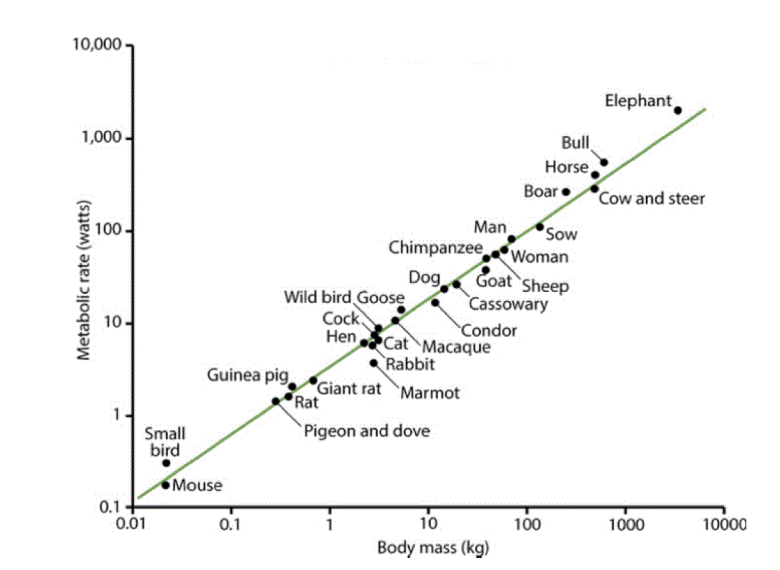
\includegraphics[width = 0.8\textwidth, angle = 0]{mouse.png}
\caption{This is the famed mouse-elephant curve, known as Kleiber's Law.}\label{fig::mouse}
\end{figure}

Go learn some philosophy! The UCO Philosophy Department is hosting a math and philosophy lecture series this fall.  The first flyer is included in Figure~\ref{fig::philosophy}.

\begin{figure}[h!]%% ! for emphasis, you are screaming "put it here!"
\centering
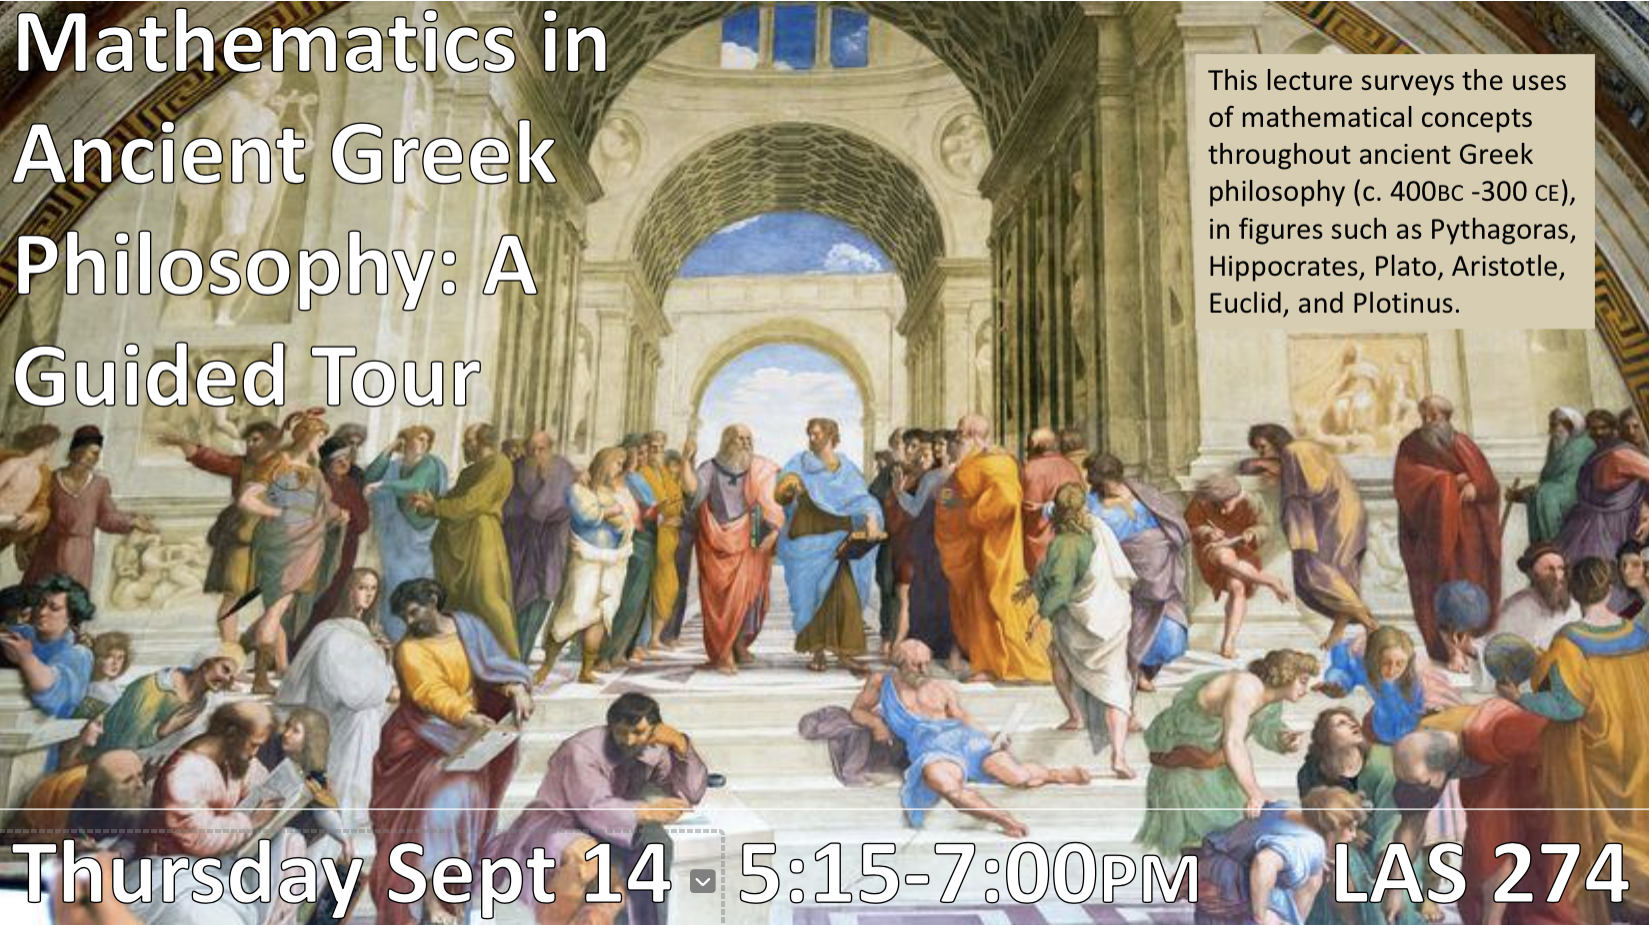
\includegraphics[width = 0.3\textwidth, angle = 0]{math-phil.png}
\caption{This is a flyer from an upcoming talk about the intersection of ancient mathematics and ancient philosophy.}\label{fig::philosophy}
\end{figure}


\begin{figure}
\begin{minipage}{0.58\textwidth}%% make sure the two numbers sum to less than one (e.g., 0.58 + 0.38)
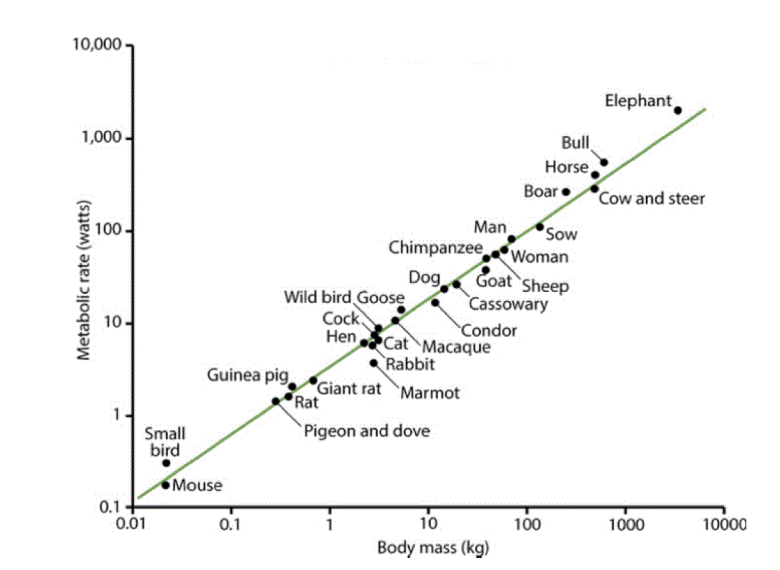
\includegraphics[width = \textwidth, angle = 0]{mouse.png}
\end{minipage}
\begin{minipage}{0.38\textwidth}
\caption{side caption. side caption. side caption. side caption. side caption. side caption. side caption. side caption.}
\end{minipage}

\end{figure}

\end{document}
